\documentclass[a4paper,11pt]{article}
\usepackage[utf8]{inputenc}
\usepackage[french]{babel} 
\usepackage[T1]{fontenc} 
\usepackage{textcomp}
\usepackage{amsmath,amssymb}
\usepackage{mathrsfs}
\usepackage{stmaryrd}
\usepackage{graphicx}
\usepackage[titlepage,fancysections]{polytechnique}

\title{SpeedTyper}
\author{Vincent DALLARD et Romain FOUILLAND}
\subtitle{Projet d'INF431}
\date{Mars 2018}


\begin{document}
\maketitle
\section{Introduction}
Le but du SpeedTyper est de taper le plus vite possible. Pour que le jeu soit pertinent, il faut donc que l'interface utilisateur (UI) soit la plus fluide possible. Ainsi, il faut gérer la vérification des mots et le décompte du temps en parallèle pour ne pas ralentir l'UI. De ce fait, un programme utilisant plusieurs threads est nécessaire.\par
Nous avons ainsi développée une première version naïve qui était gérée par l'UI. Afin d'améliorer les performances du jeu, nous avons dans une deuxième version utilisé des managers pour répartir les tâches et les nouveaux mots.\par

\section{Fonctionnement}
\subsection{Description}
La figure suivante est notre interface graphique finale.\par
\begin{center}
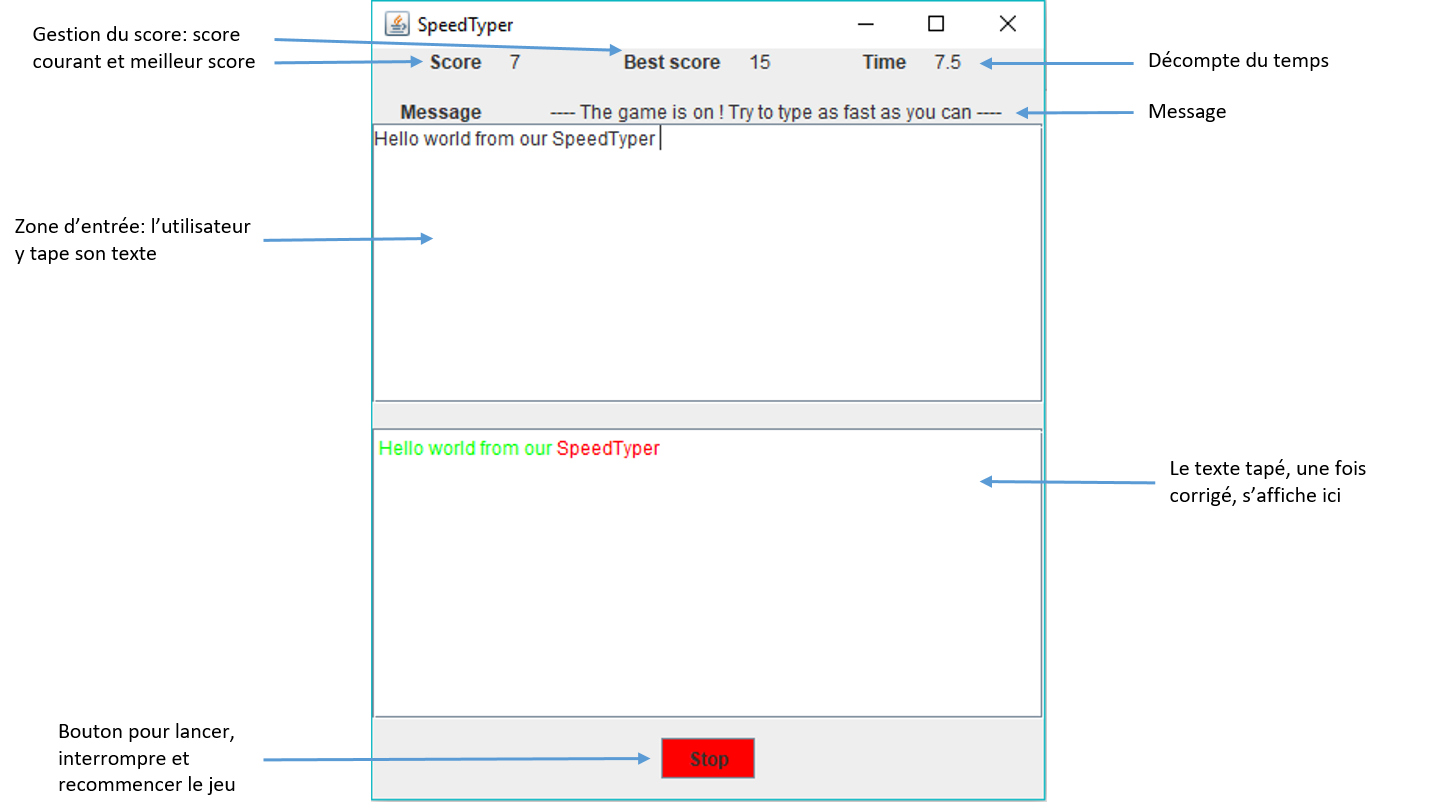
\includegraphics[width = 17cm, height = 11cm]{interfaceGraphique.png}
\end{center}\par
Comme on peut le voir, la première ligne sert à gérer les données du jeu à savoir :
\begin{itemize}
\item Le score courant du joueur
\item Le meilleur score qui est stocké dans un fichier en local pour être conservé entre les parties
\item Le temps restant avant le début du jeu ou la fin de la partie (une fois celle-ci lancée)
\end{itemize}\par
La ligne suivante permet d'afficher des messages pour donner des informations au joueur (le jeu va bientôt être lancé, le jeu est fini, en cours ou encore le meilleur score a été battu).\par
Les deux zones de texte sont la zone d'entrée où l'utilisateur pourra taper de la façon la plus fluide possible et la zone de sortie où le texte corrigé s'affiche en couleur :
\begin{itemize}
\item gris en attente de correction
\item vert si le mot existe en anglais
\item rouge s'il n'existe pas
\item bleu si c'est un nom des films célèbres
\end{itemize}
\end{document}
